%======================================================================
\NEWMOD
%======================================================================

\section{\sINTRO}

%----------------------------------------------------------------------

\logo{\hfill\hyperlink{outline<1>}{\icon}}

\begin{frame}[fragile,label=s-INTRO] 
\modframetitle{\sINTRO}
\small
\begin{center}
\begin{minipage}{3.25in}
\begin{enumerate}
\item \hyperlink{ss-purpose<1>}   {\BUTTON {\ssPurpose}}
\item \hyperlink{ss-motivation<1>}   {\BUTTON {\ssMotivation}}
\item \hyperlink{ss-compare<1>}   {\BUTTON {\ssCompare}}
\item \hyperlink{ss-approach<1>}   {\BUTTON {\ssApproach}}
\item \hyperlink{ss-issues<1>}   {\BUTTON {\ssIssues}}
%
\item \hyperlink{ss-state<1>}   {\BUTTON {\ssState}}
\item \hyperlink{ss-current<1>}   {\BUTTON {\ssCurrent}}
\item \hyperlink{ss-scaling<1>}   {\BUTTON {\ssScaling}}
%
\item \hyperlink{ss-roadmap<1>}   {\BUTTON {\ssRoadmap}}
\item \hyperlink{ss-ver-hydro<1>}   {\BUTTON {\ssVerHydro}}
\item \hyperlink{ss-ver-chemistry<1>}   {\BUTTON {\ssVerChemistry}}
\item \hyperlink{ss-ver-gravity<1>}   {\BUTTON {\ssVerGravity}}
\item \hyperlink{ss-ver-particles<1>}   {\BUTTON {\ssVerParticles}}
\item \hyperlink{ss-ver-magnetism<1>}   {\BUTTON {\ssVerMagnetism}}
\item \hyperlink{ss-ver-radiation<1>}   {\BUTTON {\ssVerRadiation}}
\item \hyperlink{ss-contribute<1>}   {\BUTTON {\ssContribute}}
%
\item \hyperlink{ss-project<1>}   {\BUTTON {\ssProject}}
\item \hyperlink{ss-documentation<1>}   {\BUTTON {\ssDocumentation}}
\item \hyperlink{ss-bugs<1>}   {\BUTTON {\ssBugs}}
\item \hyperlink{ss-testing<1>}   {\BUTTON {\ssTesting}}
\item \hyperlink{ss-source<1>}   {\BUTTON {\ssSource}}
\item \hyperlink{ss-browse<1>}   {\BUTTON {\ssBrowse}}
\item \hyperlink{ss-communicate<1>}   {\BUTTON {\ssCommunicate}}

\end{enumerate}
\end{minipage}
\end{center}
\end{frame}

\logo{\hfill\hyperlink{s-INTRO<1>}{\icon}}

%======================================================================
\NEWSEC
%======================================================================

%\subsection{\ssPurpose}

\begin{frame}[fragile,label=ss-purpose] 
\frametitle{\ssPurpose}

Three main goals:
\begin{enumerate}
\item Tell you \blueit{\textbf{what} Enzo-P is} (and \blueit{\textbf{why} it exists})
\item Help you learn to \blueit{\textbf{use} Enzo-P}
\begin{itemize}
\item download Enzo-P / Cello
\item configure / compile / run
\item write parameter files
\end{itemize}
\item Show you how to \blueit{\textbf{develop} Enzo-P}
\begin{itemize}
\item \charm\ parallel programming system
\item Cello software design
\item add parameters
\item add methods, refinement criteria
\item add initial and boundary conditions
\end{itemize}
\end{enumerate}
%Enzo-P has had a single developer for long enough. \\
%That needs to change. \\
%Today! \pause (\ldots and tomorrow)
\end{frame}

%Other material that needs to be covered:
%\begin{itemize}
%\item \blueit{Charm++} Parallel programming system
%\item Current \blueit{project organization}
%\end{itemize}
     % What is the purpose of this workshop?
%======================================================================
\NEWSEC
%======================================================================

\subsection{\ssMotivation}

\begin{frame}[fragile,label=ss-motivation] 
\secframetitle{\ssMotivation}
% One might ask why am I working on Enzo-P and Cello.  Enzo is clearly
% a very powerful code, capable of being applied to a wide range
% of problems in astrophysics and cosmology.

% [PHYSICS] This is due in part to Enzo's wide range of physics
% capabilites, from hydrodynamics and self-gravity, to cosmological
% expansion, chemistry and cooling, star formation, MHD, RHD, and so
% on.

% [METHODS] Enzo contains an even wider range of numerical methods,
% which serve to discretize and solve these equations.  Most of the
% physics capabilities in Enzo can be solved using one of multiple
% available methods, such as PPM, ZEUS or MUSCL hydrodynamics,
% Gadget, Cloudy, and Grackle chemistry and cooling, and implicit
% coupled FLD and Enzo+Moray RHD

% [DATA] All of Enzo's methods are in turn built on its parallel
% adaptive mesh refinement data structure.  Patches in the AMR
% hierarchy contain both particle data and mesh data, so both
% Lagrangian and Eularian methods are supported, as well as hybrid
% particle-mesh methods.

% [SLIDE] Together, these three layers enable Enzo to do numerical
% astrophysics.  The equations serve to mathematically approximate
% physical phenomena, the numerical methods serve to define how to
% represent required data on a computer and proceedures for finding
% numerical solutions to the equations, and the data structures serve
% to represent the actual numerical solution including all
% intermediate computations within the parallel computer.
  \framesubtitle{\enzo's strengths}
\centerline{\textbf{\only<1>{Applicable to a wide range of astrophysical/cosmological problems}
\only<2>{Implements a variety of sophisticated numerical methods}
\only<3>{Enabled by adaptive mesh refinement with particles and fields}}}
\setbeamercolor{block title}{bg=red!30,fg=black}
\begin{block}<+->{\textbf{Physics Equations}: \textit{mathematical models}}
   \textcolor{red!80!black}{
 \footnotesize
    \textbullet\ Hydrodynamics (Euler equations)
    \textbullet\ Gravity ($\nabla^2\Phi=4\pi G\rho$)
    \textbullet\ Chemistry/cooling
    \textbullet\ Star formation
    \textbullet\ Magnetism
    \textbullet\ Radiation \Large $\ldots$
    }
\end{block}

\setbeamercolor{block title}{bg=green!30,fg=black}
\begin{block}<+->{\textbf{Numerical Methods}: \textit{approximate and solve}}
    \textcolor{green!50!black}{
\footnotesize     \textbullet\ PPM, \textbullet\ ZEUS, \textbullet\ MUSCL
     \textbullet\ FFT \textbullet\ multigrid
     \textbullet\ Gadget cooling
     \textbullet\ Cloudy cooling
     \textbullet\ Grackle
     \textbullet\ Dedner MHD
     \textbullet\ MHD-CT
     \textbullet\ Implicit FLD
     \textbullet\ Moray \Large $\ldots$
     }
  \end{block}

\setbeamercolor{block title}{bg=blue!30,fg=black}
\begin{block}<+->{\textbf{Data Structures}: \textit{computer representation}}
    \textcolor{blue}{
\footnotesize
    \textbullet\ Structured Adaptive Mesh Refinement (SAMR)
    \textbullet\ Eularian fields
    \textbullet\ Lagrangian particles
 \Large $\ldots$}
  
\end{block}

\end{frame}

%-----------------------------------------------------------------------

 \begin{frame}[fragile] 

% The main thing that Enzo struggles with is keeping up with
% the continual exponential increase in parallelism in HPC
% systems.  20 years ago when Enzo was first conceived,
% typical ``massively parallel'' machines had on the order
% of 100 processors, but today's machines have thousands times
% more cores.

% The physics is relatively untouched.  We still want to solve the
% same equations we did 20 years ago.  The numerical methods are also
% mostly the same--hydrodynamics/chemistry are local, FFT's and
% multigrid require some changes but still viable.  The main effect is
% on Enzo's parallel AMR data structures.  AMR meta data didn't used
% to be a problem, but it's a hard limit on scalability now.
% Hierarchy overhead wasn't a problem when it had to loop over
% hundreds of grids, but now it is when it has to loop over millions.
% As hardware parallelism increases, Enzo runs into bottleneck after
% bottleneck, in both memory usage and parallel computation.  Even MPI
% as used in Enzo has limits---barriers and other global operations
% become increasingly costly as core counts increase

% This is what motivated me to start working on Enzo-P/Cello.
% The idea was to redesign and implement the AMR data structure
% from scratch to be as scalable as possible, targeting machines
% that didn't even exist when the project started.  This AMR
% data structure is in a separate reusable framework called Cello.
% Enzo-P is the port of Enzo's physics and numerical methods onto
% Cello.

%---------
% SLIDE 2
%---------

% That's a summary of Enzo's strengths.  Enzo has limitations as well,
% and they are primarily due to the vast increase in size and
% complexity of the high performance computer hardware we have access
% to.  Development on Enzo began about 20 years ago, when ``massively parallel''
% meant about 100 processors.  Today, supercomputers can contain
% a hundred *thousand* processors.  This has affected the three conceptual layers of 
% Enzo in different ways.

% [PHYSICS] The higher-level mathematical equations defining the physics
% are mostly unchanged.  The equations for hydrodynamics and gravity are the
% same today as they were 20 years ago.  Enzo has certainly increased
% its range of problems it can solve, for example by adding support for MHD and RHD,
% but the existing physics requirements are unchanged.

% [METHODS] Numerical methods in Enzo are still very usable for the
% most part.  Methods for solving localized physics such as
% hydrodynamics and chemistry and cooling have the same requirements
% as 20 years ago, and those for global physics such as self-gravity
% are based on FFT's and multigrid, which are still usable on todays
% supercomputers, though may require some optimizations in terms of
% structuring the data

% [DATA STRUCTURES] Which brings us to data structures.  Of these
% three, supercomputer growth has affected the usability of Enzo's
% data structures the most.  Unfortunately, they're also the most
% difficult to change, since all of Enzo's numerical methods use them,
% and changing any part of how Enzo does AMR can lead to a global
% effect on the code.

% [ENZO-P] This is why several years ago I started working on Enzo-P
% and Cello.  Enzo-P serves to contain the physics capabilities and
% numerical methods in Enzo, whereas Cello serves to implement a
% totally new AMR framework designed to be highly scalable, capable of
% running on petascale and ultimately exascale machines.  Needless to
% say, designing software to run on classes of machines that don't
% exist yet is difficult, though a lot of thought has been put into
% making Cello as scalable as possible, so that Enzo's physics can
% continue to live and thrive for many years to come.

\secframetitle{\ssMotivation}
%  \framesubtitle{\enzo's struggles}
 \centerline{\textbf{ENZO has difficulties scaling to modern HPC platforms}} \ \\
 \begin{minipage}{3in}
\pause
  \begin{itemize}
   \item Ever-changing software requirements
     \begin{itemize}
\footnotesize
   \item  Enzo was born in early 1990's
   \item ``massive parallelism'' meant $P\approx 100$
   \item $\times 10^5$ parallelism today
     \end{itemize}
   
\pause
   \item Affects different parts of \enzo\ differently
     \begin{itemize}
   \item[\smiley] \textcolor{red!80!black}{physics} requirements unchanged
   \item[\smiley] \textcolor{green!50!black}{numerical methods} mostly viable
   \item[\frownie] \textcolor{blue}{\textit{data structures}} limit Enzo's scalability
     \end{itemize}
\pause
   \item Motivates AMR data structure redesign
   \begin{itemize}
   \footnotesize
   \item  \textbf{\enzop}: ``petascale'' version of \enzo
   \item keep \enzo's \textcolor{red!80!black}{physics} and many \textcolor{green!50!black}{methods}
   \item  built on \textbf{\cello} \textcolor{blue}{scalable AMR framework}
   \end{itemize}
  \end{itemize}
\end{minipage}
\begin{minipage}{1in}
   \footnotesize
    \centerline{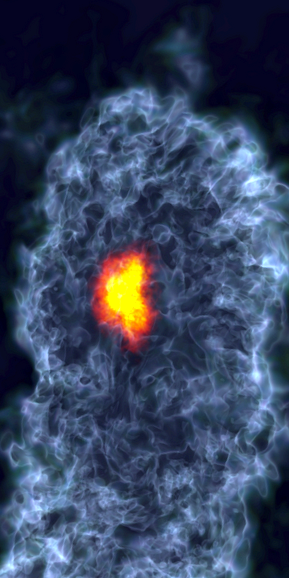
\includegraphics[width=0.875in]{PopIII_vr-edit.png}}
    \centerline{\tiny {[ Sam Skillman, Matt Turk ]}}
\end{minipage}
\end{frame}

  % Why does Enzo-P exist?
%======================================================================
\NEWSEC
%======================================================================

\subsection{\ssCompare}

\usebackgroundtemplate
{
\includegraphics[width=5in]{cello-background.png}}
\begin{frame}[fragile,label=ss-compare] 
% ----------------------------------------------------------------------
\secframetitle{\ssCompare}
%\framesubtitle{}
% ----------------------------------------------------------------------
\begin{center}
\rowcolors[]{1}{blue!5}{blue!10}
\begin{tabular}{l|cc} 
 & \textbf{\enzo} & \textbf{\enzopcello} \\ \hline
\uncover<2->{Parallelization} & \uncover<2->{MPI} & \uncover<2->{\charm} \\
\uncover<3->{AMR type}       & \uncover<3->{patch-based} & \uncover<3->{octree-based}   \\
\uncover<4->{AMR structure} & \uncover<4->{replicated} &\uncover<4->{ fully distributed}   \\
\uncover<5->{Time stepping} & \uncover<5->{level-adaptive} & \uncover<5->{block-adaptive$^*$}   \\
\uncover<6->{Block sizes} & \uncover<6->{$\times 1000$ variation} & \uncover<6->{constant}  \\
\uncover<7->{Task scheduling} & \uncover<7->{level-parallel} & \uncover<7->{dependency-driven}  \\
\uncover<8->{Load balancing} & \uncover<8->{patch migration} & \uncover<8->{\charm-based}  \\
\uncover<9->{Data locality} & \uncover<9->{LB conflict} & \uncover<9->{no LB conflict}  \\ 
\uncover<10->{Mesh quality} & \uncover<10->{level jumps} & \uncover<10->{2-to-1 constraint}  \\  \hline
\end{tabular} \\
\uncover<5->{\footnotesize $^*$ not implemented yet}
%  
% \ \\ \ \\
% \url{http://cello-project.org} \\
% NSF PHY-1104819, AST-0808184 \\
% $\qed$
\end{center}
\end{frame}

\usebackgroundtemplate
{}
     % What are the key differences between Enzo-P and Enzo?
%======================================================================
\NEWSEC
%======================================================================

\subsection{\ssApproach}

\begin{frame}[fragile,label=ss-approach] 
\secframetitle{\ssApproach}
\framesubtitle{\enzo's limitations}
%\framesubtitle{Scaling issues}
\begin{minipage}{3.0in}
%  AMR data structure scalability
%  Code development and maintenance
%  Ghost zone memory requirement
%  Patch size variation
%  Time stepping
%  Dynamic load balancing
%  Particle positions
%  Mesh quality
% So, how does Cello's AMR try to address the know issues of Enzo's current
% AMR?
%
% The main issues with Enzo's AMR design and implementation involve
% memory usage, the quality of the mesh, parallel task definition
% and scheduling, and data locality.

% [MEMORY] Memory usage is perhaps the most common limitation that
% people run into when running big Enzo simulations.  Enzo's mesh
% hierarchy structure is represented in each MPI process using a
% grid object for each AMR patch.  Although patches assigned to
% remote processors carry no field or particle data, the grid
% objects themselves still take up on the order of a few KB of memory.
% For small hierarchies that's not a problem, but when you have a million
% grid patches that means several GB of memory are required on each
% MPI process.  While supercomputers have gotten larger over the years, the
% amount of memory per node has not---it's still frequently just a few
% GB.  :  Memory fragmentation has also been identified as a problem,
% due to the high volume of heap memory new and delete operations on
% widely varying array sizes.  Ghost zone data can also consume a lot
% of memory, especially for smaller grids.

% [ MESH QUALITY ] Enzo also has known mesh quality issues.  Sometimes
% patches are adjacent to patches in refinement levels that are further than 
% a factor of two different. This can lead to inaccurate interpolation
% compromizing the numerical accuracy of solutions on such patches.

% [ PARALLEL TASKS ] Parallel tasks in Enzo are defined as a grid
% object and its associated field and particle data.  Patch sizes in
% Enzo can vary widly, from large $64^3$ root grid tiles to small
% $8^3$ patches on the finest levels.  Varying task sizes can
% adversely affect performance and load balancing.

\begin{itemize}
\item \bfat{2}{\textcolor{red!50!black}{Memory usage}}
\begin{itemize}
  \item<2-> \textcolor{red}{AMR structure is non-scalable}
  \item<2-> \textcolor{red}{memory fragmentation}
  \item<2-> \textcolor{red}{ghost zones}
\end{itemize}
\item \bfat{3}{\textcolor{green!50!black}{Mesh quality}}
\begin{itemize}
   \item<3-> \textcolor{green!80!black}{2-to-1 refinement constraint violated}
\end{itemize}
\item \bfat{4}{\textcolor{blue!50!black}{Parallel task definition}}
\begin{itemize}
   \item<4-> \textcolor{blue}{widely varying patch sizes}
   \item<4-> \textcolor{blue}{sizes determined by AMR}
\end{itemize}
\item \bfat{5}{\textcolor{cyan!50!black}{Parallel task scheduling}}
\begin{itemize}
   \item<5-> \textcolor{cyan!80!black}{parallel within a level}
   \item<5-> \textcolor{cyan!80!black}{synchronization between level time steps}
\end{itemize}
\item \bfat{6}{\textcolor{orange!50!black}{Data locality}}
\begin{itemize}
   \item<6-> \textcolor{orange!80!black}{disrupted by load balancing}
\end{itemize}
\end{itemize}
\end{minipage} \
\begin{minipage}{1.0in}
\centerline{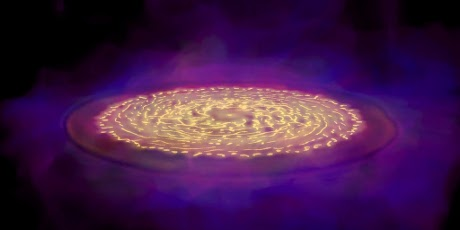
\includegraphics[width=2.0in,angle=90]{iso_and_volume_02_sm.jpg}}
\centerline{\tiny{[ Elizabeth Tasker ]}}
\end{minipage}
\end{frame}

%--------------------------------------------------

\begin{frame}[fragile] 
\secframetitle{\ssApproach}
\framesubtitle{\enzopcello\ approach}
%\framesubtitle{Scaling issues}
\begin{minipage}{3.0in}
%  AMR data structure scalability
%  Code development and maintenance
%  Ghost zone memory requirement
%  Patch size variation
%  Time stepping
%  Dynamic load balancing
%  Particle positions
%  Mesh quality
\begin{itemize}
\item \bfat{2}{\textcolor{red!50!black}{Memory usage}}
\begin{itemize}
  \item<2-> \textcolor{red}{AMR structure is fully distributed}
  \item<2-> \textcolor{red}{uniform blocks reduce fragmentation}
  \item<2-> \textcolor{red}{ghost zones allocated when needed$^*$}
\end{itemize}
\item \bfat{3}{\textcolor{green!50!black}{Mesh quality}}
\begin{itemize}
   \item<3-> \textcolor{green!80!black}{2-to-1 refinement constraint maintained}
\end{itemize}
\item \bfat{4}{\textcolor{blue!50!black}{Parallel task definition}}
\begin{itemize}
   \item<4-> \textcolor{blue}{uniform field array sizes in blocks}
   \item<4-> \textcolor{blue}{sizes determined by user}
\end{itemize}
\item \bfat{5}{\textcolor{cyan!50!black}{Parallel task scheduling}}
\begin{itemize}
   \item<5-> \textcolor{cyan!80!black}{asynchronous, data-driven}
   \item<5-> \textcolor{cyan!80!black}{block-local time stepping$^*$}
\end{itemize}
\item \bfat{6}{\textcolor{orange!50!black}{Data locality}}
\begin{itemize}
   \item<6-> \textcolor{orange!80!black}{only nearest-neighbor communication}
\end{itemize}
\end{itemize}
\vspace{-0.1in}
\only<1>{\textcolor{white}{\footnotesize $^*$ not implemented yet}}
\only<2-4>{\textcolor{red}{\footnotesize $^*$ not implemented yet}}
\only<5-6>{\textcolor{cyan!80!black}{\footnotesize $^*$ not implemented yet}}
\end{minipage} \
\begin{minipage}{1.0in}
\vspace{-0.2in}
\centerline{\tiny{Enzo}} 
\vspace{0.1in}
\centerline{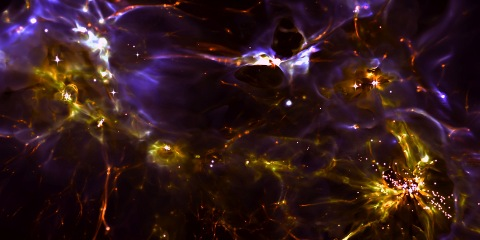
\includegraphics[width=2.0in,angle=90]{jhw-dwarf-galaxies.jpg}}
\centerline{\tiny{[ John Wise ]}}
\end{minipage}
\end{frame}

% ----------------------------------------------------------------------
    % How does Enzo-P AMR address Enzo's limitations?}
%======================================================================
\NEWSEC
%======================================================================

\subsection{\ssIssues}

\begin{frame}[fragile,label=ss-issues] 
\secframetitle{\ssIssues}
\framesubtitle{Parameter file issues}
% Review ss-bugs.tex / http://client64-249.sdsc.edu/cello-bug

\begin{itemize}
   \item Floats and ints cannot be mixed
   \cornersize{0.9}
   \begin{itemize}
     \item[\frownie] \textcolor{red}{\code{velocity\_x = 8.0 + 2*x }}
     \item[\smiley] \textcolor{green!50!black}{\code{velocity\_x = 8.0 + 2.0*x}}
   \end{itemize}

   \item Need space after subtraction minus sign
   \begin{itemize}
     \item[\frownie] \textcolor{red}{\code{density = x -2.0;}}
     \item[\smiley] \textcolor{green!50!black}{\code{density = x - 2.0;}}
   \end{itemize}
  \item Need at least as many root blocks as processors $P$
  \begin{itemize}
    \item \code{Mesh \{ root\_blocks = [4,4,4]; \} }
    \item[\frownie] \textcolor{red}{\code{\$ charmrun +p72} \code{bin/enzo-p \ldots}}
    \item[\smiley]\textcolor{green!50!black}{\code{\$ charmrun +p64} \code{bin/enzo-p \ldots}}
  \end{itemize}
  \item AMR requires ghost zone depth of $\ge 4$
\end{itemize}

\link{ss-bugs}{Other issues: see bug tracking website}

\end{frame}
      % What are some of Enzo-P's known issues?
%
%======================================================================
\NEWSEC
%======================================================================

\subsection{\ssState}

\begin{frame}[fragile,label=ss-state] 

\secframetitle{\ssState}

%  What is the current state of Enzo-P?  Well, it can do this.

%  This is a pure hydrodynamics problem run using Enzo-P with AMR
%  enabled, with somewhat non-physical initial conditions.

%  It uses an ``array of octrees'' AMR approach, which is simply a
%  uniform array of octrees.  Each Block in the hierarchy contains a
%  small grid of field variables, with size typically around 16^3 to
%  32^3.

%  Enzo-P is parallelized using Charm++ instead of MPI.  Charm++ is an
%  asynchronous data-driven parallel programming language extention to
%  C++.  Each block in the mesh hierarchy is a separate parallel task
%  in Charm, called called a ``chare''.  A key feature of Cello's AMR
%  Charm++ implementation is that it is fully distributed--there is
%  *no* hierarchy meta-data, which addresses a key limitation of
%  the current Enzo.

%  Enzo-P is also designed to be powerful yet easy to use.  While you
%  *can* implement test problem types in Enzo-P like you can Enzo, you
%  can also specify initial and boundary conditions directly in the
%  parameter file.  In this example, initial conditions were generated
%  using a PNG file as a logical mask---the density is initialized to
%  1.5 wherever the PNG file pixels are non-black, otherwise its set
%  to be 12 times less.  This approach means that common test problems
%  such as the implosion problem, Sedov blast wave, or double mach
%  reflection can be set up in the parameter file exclusively without
%  requiring any C++ coding.

\pause
\begin{center}
\begin{minipage}{4.5in}
\begin{minipage}{2.9in}
\only<2->{\vspace{-0.1in}\centerline{in 2014} \ \\ \vspace{-0.2in} \ANIMATEGRAPHICS{width=2.9in}{10}{Images/Daze/daze-0}{000}{100}}
\end{minipage} \ 
\begin{minipage}{1.45in}
\only<3->{\vspace{-0.1in}\centerline{in 2015} \ \\ \vspace{-0.2in}\ANIMATEGRAPHICS{width=1.45in}{10}{Images/1509/1509-0}{00}{56}}
\end{minipage}
\end{minipage}
\end{center}
\pause
\pause
\begin{minipage}[t]{1.2in}
\footnotesize
\vspace{0.1in}
\blockred
\begin{block}<+->{\textbf{Mesh refinement}}
\scriptsize
 \mbox{``array-of-octrees''} \\
 \mbox{field data on blocks} \\ \ \\
\end{block}
\end{minipage} \ \ 
\begin{minipage}[t]{1.0in}
\footnotesize
\vspace{0.1in}
\blockgreen
\begin{block}<+->{\textbf{Parallelism}}
\scriptsize
 Charm++\\
\mbox{blocks are ``chares''} \\
 \mbox{fully-distributed}
\end{block}
\end{minipage} \ \
\begin{minipage}[t]{1.6in}
\raggedright
\footnotesize
\vspace{0.1in}
\blockblue
\begin{block}<+->{\textbf{Parameters}}
\scriptsize
 \mbox{\code{Initial \{ density \{}} \\
 \mbox{\code{ value = [ 1.5, "daze.png",  }} \\
 \mbox{\code{\ \ \ \ \ \ \ \ \ \ \ 0.125 ]; \} \} }}
\end{block}
\end{minipage}

\end{frame}

%----------------------------------------------------------------------

\begin{frame}[fragile,label=ss-state] 
\secframetitle{\ssState}
\begin{center}
\begin{minipage}{4.5in}
\begin{minipage}{2.2in}
\only<2->{\centerline{in 2016}}
\end{minipage}
\begin{minipage}{2.2in}
\only<3->{\centerline{in 2017}}
\end{minipage}
 \vspace{0.2in} \\
\begin{minipage}{2.2in}
\begin{center}
\only<2->{\ANIMATEGRAPHICS{width=1.8in}{10}{trace-}{00}{99}}
\end{center}
\end{minipage} \
\begin{minipage}{2.2in}
\only<3->{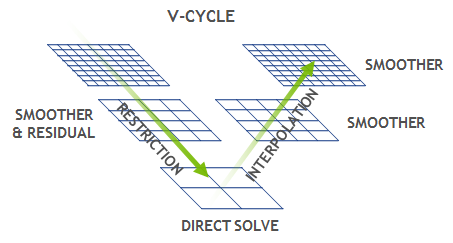
\includegraphics[width=2.0in]{hpgmg_v_cycle.png}}
\end{minipage}
\end{minipage}
\end{center}
\end{frame}

%----------------------------------------------------------------------

\begin{frame}[fragile,label=ss-state] 
\secframetitle{\ssState}
\begin{center}
\centerline{in 2018}  \ \\
\begin{minipage}{4.5in}
\begin{minipage}{2.2in}
\only<2->{\ANIMATEGRAPHICS{width=2.0in}{5}{Images/Cosmo/B3/dark-}{00}{21}}
\end{minipage} \
\begin{minipage}{2.2in}
\only<3->{\ANIMATEGRAPHICS{width=2.0in}{5}{Images/Cosmo/B3/mesh-}{00}{21}}
\end{minipage}
\end{minipage}
\end{center}
\end{frame}

  % What is the current state of Enzo-P/Cello?
%======================================================================
\NEWSEC
%======================================================================

\subsection{\ssCurrent}

% ----------------------------------------------------------------------
\begin{frame}[fragile,label=ss-current] 
\secframetitle{\ssCurrent}

\rowcolors[]{1}{blue!5}{blue!10}
\begin{tabular}{ll}
\uncover<2->{\erow{Physics}} &
\uncover<2->{\erow{PPM, \magentabf{scalable} gravity, (grackle), \magentabf{cosmology}}} \\

\uncover<3->{\orow{Field data}} &
\uncover<3->{\orow{(padding, alignment, precision, centering)}} \\

\uncover<4->{\erow{Particle data}} &
\uncover<4->{\erow{(types, attributes, batches, constants)}} \\

\uncover<5->{\orow{Initial conditions}} &
\uncover<5->{\orow{direct ($f(x,y,z)$), problems (Implosion, Sedov)}} \\

\uncover<6->{\erow{Boundary conditions}} &
\uncover<6->{\erow{inflow ($f(x,y,z,t)$), outflow, reflecting, periodic}} \\

\uncover<7->{\orow{Refinement criteria}} &
\uncover<7->{\orow{slope, density, shear, shock, \magentabf{mass}}} \\

\uncover<8->{\erow{Interpolation}} &
\uncover<8->{\erow{linear, \textcolor{gray}{\enzo's \textit{SecondOrderA}, etc.}}} \\

\uncover<9->{\orow{Time stepping}} &
\uncover<9->{\orow{uniform, \textcolor{gray}{level-adaptive}, \textcolor{gray}{block-adaptive}}} \\

\uncover<10->{\erow{Checkpoint/restart}} &
\uncover<10->{\erow{\charm\ (disk, memory+disk)}} \\

\uncover<11->{\orow{Load balancing}} &
\uncover<11->{\orow{\charm\ (dozens of strategies available)}} \\

\uncover<12->{\erow{I/O}} &
\uncover<12->{\erow{\textcolor{gray}{scalable} HDF5, PNG}} \\
\end{tabular}
\ \\
\ \\
\ \\
\centerline{
\uncover<1->{\magentatext{New capability}} \hfill
\uncover<1->{\bluetext{Pre-existing capability}} \hfill
\uncover<1->{\textcolor{gray}{Not ready yet}}}
\end{frame}
  % What are Enzo-P's current and near future capabilities?
%======================================================================
\NEWSEC
%======================================================================

\subsection{\ssScaling}

\begin{frame}[fragile,label=ss-scaling] 
\secframetitle{\ssScaling}
\begin{center}
\begin{minipage}{4.50in}
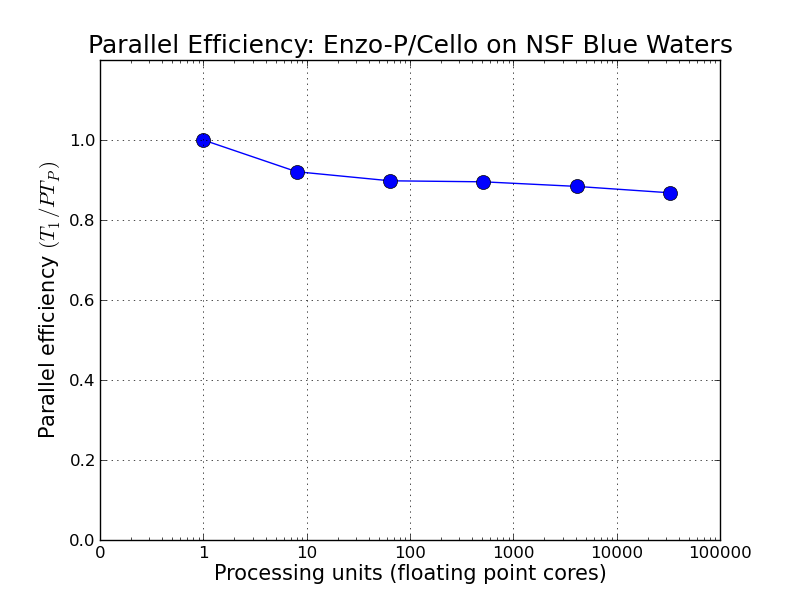
\includegraphics[width=2.25in]{scale-eff.png} \ 
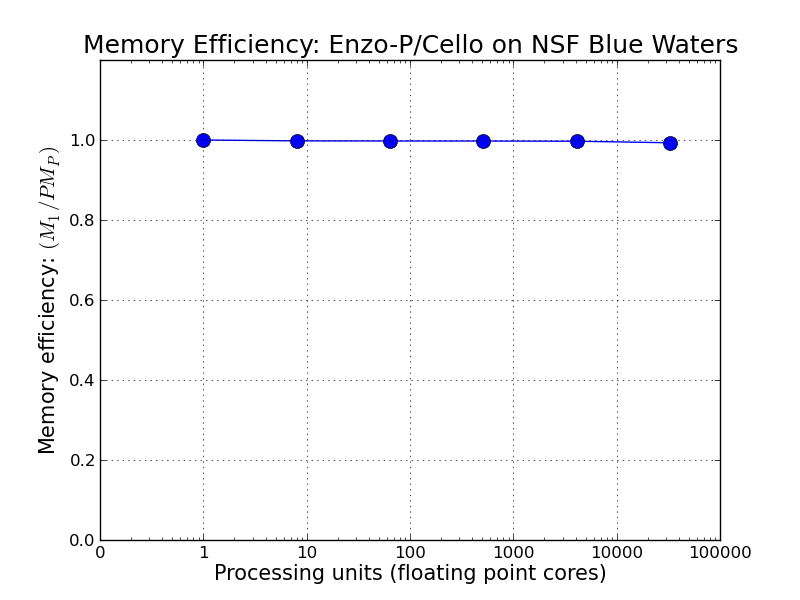
\includegraphics[width=2.25in]{scale-mem.png}
\end{minipage} \\
\begin{minipage}{4.0in}
\footnotesize
\pause
\begin{minipage}[t]{1.20in}
\blockblue
\begin{block}<+->{Problem}
%\begin{itemize}
Sedov blast array \\
$L=3$; $32K$ cores \\
$32^3$ cells / block \\
$329$ blocks /core
%\end{itemize}
\end{block}
\end{minipage} \
\begin{minipage}[t]{1.20in}
\blockgreen
\begin{block}<+->{Parallel Efficiency}
%\begin{itemize}
\begin{tabbing}
xxxxxxxxxx\=\kill
Time \> $0.868$ \\
Memory \> $0.993$
\end{tabbing}
%\end{itemize}
\end{block}
\end{minipage} \
\begin{minipage}[t]{1.20in}
\blockred
\begin{block}<+->{Caveats}
%\begin{itemize}
load balanced \\
few refinement steps \\
startup ignored
%\end{itemize}
\end{block}
\end{minipage}
\end{minipage}
\end{center}
\end{frame}

  % How well does ENzo-P scale?
%
%======================================================================
\NEWSEC
%======================================================================

\subsection{\ssRoadmap}

\begin{frame}[fragile,label=ss-roadmap] 
\secframetitle{\ssRoadmap}
%\framesubtitle{(Contingent on funding)}
\scriptsize
%\newcommand{\alignbox}[2]{\makebox[1.75in][l]{#2: \textbf{#1}}}
\newcommand{\alignbox}[2]{}
\blockblue
\textbf{\ \\ This preliminary roadmap may change based on \enzo\ community requests}
\begin{center}
\begin{minipage}{4.5in}
\begin{minipage}{2.0in}
\setbeamercolor{block title}{bg=green!30,fg=black}
\begin{block}<1->{\textbf{Month 00:} Version 1.0 (\textit{hydro})}
\scriptsize
\textcolor{enzop}{(10\%) beta testing} \\
\textcolor{cello}{(80\%) fix bugs, optimize performance}
\end{block}
\end{minipage} \ 
\setbeamercolor{block title}{bg=blue!30,fg=black}
\begin{minipage}{2.0in}
\begin{block}<4->{\textbf{Month 18:} Version 4.0 (\textit{particles})}
\scriptsize
\textcolor{enzop}{ migrate PM, implement P$^3$M / TreePM} \\
\textcolor{cello}{ ``face-methods'' for MHD}
\end{block}
\end{minipage}
\end{minipage} \\
\begin{minipage}{4.5in}
\begin{minipage}{2.0in}
\setbeamercolor{block title}{bg=green!30,fg=black}
\begin{block}<2->{\textbf{Month 06:} Version 2.0 (\textit{chemistry})}
\scriptsize
\textcolor{enzop}{(70\%) chemistry solvers} \\
\textcolor{cello}{(70\%) linear solvers, adaptive time steps}
\end{block}
\end{minipage} \ 
%\setbeamercolor{block title}{bg=blue!30,fg=black}
\begin{minipage}{2.0in}
\setbeamercolor{block title}{bg=blue!30,fg=black}
\begin{block}<5->{\textbf{Month 24:} Version 5.0 (\textit{magnetism})}
\scriptsize
\textcolor{enzop}{migrate \enzo\ MHD methods to \enzop} \\
\textcolor{cello}{adaptive ray tracing support}
\end{block}
\end{minipage}
\end{minipage} \\
\begin{minipage}{4.5in}
\begin{minipage}{2.0in}
\setbeamercolor{block title}{bg=green!30,fg=black}
\begin{block}<3->{\textbf{Month 12:} Version 3.0 (\textit{gravity})}
\scriptsize
\textcolor{enzop}{(50\%) cosmological self-gravity, coupled-implicit FLD RT} \\
\textcolor{cello}{(20\%) particles, optimize linear solvers}
\end{block}
\end{minipage} \ 
\begin{minipage}{2.0in}
\setbeamercolor{block title}{bg=blue!30,fg=black}
\begin{block}<6->{\textbf{Month 36:} Version  6.0 (\textit{radiation})}
\scriptsize
\textcolor{enzop}{\enzo+Moray RHD} \\
\textcolor{cello}{optimize performance and scalability} \\
\end{block}
\end{minipage}
\end{minipage}
\ \\
\ \\
\centerline{\textcolor{enzop}{Red: Enzo-P}}
\centerline{ \textcolor{cello}{Green: Cello}}
\end{center}

%\end{quotation}

% Weeks
% \begin{itemize}
%   \item Dynamic load balancing via \charm
%   \item Parallel checkpoint/restart
%   \item Grackle chemistry/cooling
%   \item MHD
% \end{itemize}
% Few Months
% \begin{itemize}
% \item self-gravity
% \item particles
% \item 
% \end{itemize}
% Many Months
% 
% 
% Ray tracing
% 
% 
% Methods: chemistry/cooling, cosmology, gravity, MHD, radiation
% Block Data: particles
% Initial conditions: problem generator, specified with masks
% Boundary conditions: inflow,outflow,reflecting,periodic with masks
% Refinement: slope
% Parallelism: Charm++, Simulation processor group, CommBlock chare array
% I/O
%    PNG, HDF5
%    Checkpoint / Restart: P>1
\end{frame}

 % What is the project roadmap?
%======================================================================
\NEWSEC
%======================================================================

\subsection{\ssVerHydro}

\begin{frame}[fragile,label=ss-ver-hydro] 
\secframetitle{\ssVerHydro}

\begin{center}
\begin{minipage}{3.6in}
\begin{enumerate}
\item[$\bigcirc$] \highpriority\  \redtext{Adaptive time-stepping}
\begin{itemize}
\item \redtext{flux correction}
\item \redtext{interpolation in time}
\end{itemize}
\item[\redcirc] \highpriority\  \redtext{Conservative interpolation}
\item[\redcirc] \highpriority\  \redtext{Bug \#60: sporatic failures if DLB enabled}
\pause
\item[\orangecirc] \medpriority\  \orangetext{Bug \#19: changing blocking changes results}
\item[\orangecirc] \medpriority\  \orangetext{More rigorous hydro tests}
\begin{itemize}
\item[\smiley] \orangetext{have implosion, sedov blast, double-mach, collapse}
\item[\frownie] \orangetext{no 1D test problems}
\end{itemize}
\item[\orangecirc] \medpriority\  \orangetext{More Riemann solvers}
\pause
\item[\greencirc] \lowpriority\  \greentext{CUDA hydro solver}
\item [\greencirc] \lowpriority\  \greentext{Performance optimization}
\item[\greencirc] \lowpriority\  \greentext{ZEUS hydro}
\end{enumerate}
\end{minipage}
\end{center}

\end{frame}

 % What is needed to complete V1.0 (hydrodynamics)?
%======================================================================
\NEWSEC
%======================================================================

\subsection{\ssVerChemistry}

\begin{frame}[fragile,label=ss-ver-chemistry] 
\secframetitle{\ssVerChemistry}
\begin{center}
\begin{minipage}{3.6in}
\begin{enumerate}
\item[\redcirc] \highpriority\ \redtext{Input remaining Grackle parameters}
\item[\redcirc] \highpriority\  \redtext{Rigorous chemistry / cooling tests}
\pause
\item[\orangecirc] \medpriority\ \orangetext{Update Grackle code to be \charm -friendly}
\begin{itemize}
\item \orangetext{write} \orangecode{::pup()} \orangetext{methods for grackle structs / classes}
\item \orangetext{required for dynamic load-balancing}
\item \orangetext{required for checkpoint / restart}
\end{itemize}
\item[\orangecirc] \medpriority\ \orangetext{Update to more recent Grackle version}
\pause
\item[$\bigcirc$] \ldots ?
\end{enumerate}
\end{minipage}
\end{center}

\end{frame}

 % What is needed to complete V2.0 (chemistry)?
%======================================================================
\NEWSEC
%======================================================================

\subsection{\ssVerGravity}

\begin{frame}[fragile,label=ss-ver-gravity] 
\secframetitle{\ssVerGravity}
%\item[$\bigcirc$] \verb@[#B]@ Cosmology

\begin{center}
\begin{minipage}{3.8in}
\begin{enumerate}
\item[\redcirc] \highpriority\ 
\redtext{Debug \texttt{Mg0} root-level multigrid solver}
\item[\redcirc] \highpriority\ 
\redtext{Incorporate \texttt{Mg0} as preconditioner to \texttt{BiCGStab}}
\item[\redcirc] \highpriority\ 
\redtext{Implement scalable multigrid solver}
\pause
\item[\orangecirc] \medpriority\ \orangetext{Optimize ghost-referesh}
\begin{itemize}
\item \orangetext{70\% time spent in \code{FieldFace} methods}
\item \orangetext{excessive mallocs and data copies}
\item \orangetext{sends ghost zones for all fields (Bug \#76)}
\item \orangetext{global barrier each refresh}
\end{itemize}
\pause
\item[\greencirc] \lowpriority\ \greentext{Separate gravity (physics) from solver (method)}
\begin{itemize}
\item \greentext{currently \code{EnzoMethodGravityCg}}
\item \greentext{change to \code{EnzoPhysicsGravity}, \code{EnzoSolverCg}}
\end{itemize}

\end{enumerate}
\end{minipage}
\end{center}
\end{frame}

 % What is needed to complete V3.0 (gravity)?
%======================================================================
\NEWSEC
%======================================================================

\subsection{\ssVerParticles}

\begin{frame}[fragile,label=ss-ver-particles] 
\secframetitle{\ssVerParticles}

\begin{center}
\begin{minipage}{3.8in}
\begin{enumerate}
\item [\redcirc] \highpriority\ \redtext{Finish ParticleBlock, ParticleDescr classes}
\begin{itemize}
\item \redtext{particle positions relative using integers}
\item \redtext{\code{kick()} and \code{drift()} methods}
\item \redtext{particle groups}
\item \redtext{particle attributes}
\end{itemize}
\item [\redcirc] \highpriority\ \redtext{\texttt{ParticleFace} support for ghost region refresh}
\item [\redcirc] \highpriority\ \redtext{Communicating particles between processes}
\pause
\item [\orangecirc] \medpriority\ \orangetext{Particle I/O}
\pause
\item[$\bigcirc$] \ldots ?
\end{enumerate}
\end{minipage}
\end{center}
   
\end{frame}

 % What is needed to complete V4.0 (particles)?
%======================================================================
\NEWSEC
%======================================================================

\subsection{\ssVerMagnetism}

\begin{frame}[fragile,label=ss-ver-magnetism] 
\secframetitle{\ssVerMagnetism}
\begin{center}
\begin{minipage}{3.6in}
\begin{enumerate}
\item[\redcirc] \highpriority\ \redtext{Face-methods}
\item[\redcirc] \highpriority\ \redtext{Port Enzo MHD methods to Enzo-P}
\pause
\item[$\bigcirc$] \ldots ?
\end{enumerate}
\end{minipage}
\end{center}
\end{frame}

 % What is needed to complete V5.0 (magnetism)?
%======================================================================
\NEWSEC
%======================================================================

\subsection{\ssVerRadiation}

\begin{frame}[fragile,label=ss-ver-radiation] 
\secframetitle{\ssVerRadiation}
\begin{center}
\begin{minipage}{3.6in}
\begin{enumerate}
\item[\redcirc] \highpriority\ \redtext{FLD solver}
\item[\redcirc] \highpriority\ \redtext{Shooting rays} \ \\
\centerline{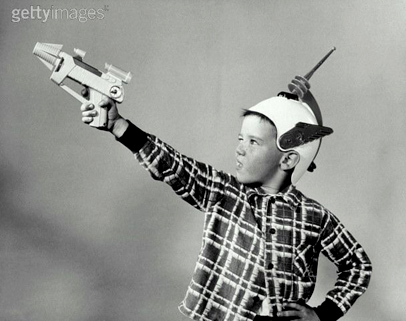
\includegraphics[width=2.0in]{Images/remco_gun_boy2.jpg}}
\item[\redcirc] \highpriority\ \redtext{Interface with Moray}
\pause
\item[$\bigcirc$] \ldots ?
\end{enumerate}
\end{minipage}
\end{center}
\end{frame}

 % What is needed to complete V6.0 (radiation)?
%======================================================================
\NEWSEC
%======================================================================

\subsection{\ssContribute}

\begin{frame}[fragile,label=ss-contribute] 
\label{frame:help}
\secframetitle{\ssContribute}
\textbf{Thanks for asking!} \\ \ \\
\begin{minipage}{4.5in}
\begin{center}
\rowcolors[]{1}{blue!5}{blue!10}
\begin{tabular}{rl}
\uncover<1->{\orow{\textbf{Beta User}}} &
  \uncover<1->{\orow{download and experiment with \enzop}} \\
  \uncover<2->{\orow{\textbf{Testing}}} &
  \uncover<2->{\orow{develop and submit test problems}} \\
  \uncover<3->{\erow{\textbf{Debugging}}} &
  \uncover<3->{\erow{help track down and fix bugs}} \\
  \uncover<4->{\orow{\textbf{Documentation}}} &
  \uncover<4->{\orow{write or update documentation}} \\
  \uncover<5->{\erow{\textbf{Developing}}} &
  \uncover<5->{\erow{migrate \enzo\ physics capabilities to \enzop }} \\
  \uncover<6->{\erow{\textbf{Refactoring}}} &
  \uncover<6->{\erow{refactor uglier or more complicated code sections}} \\
  \uncover<7->{\orow{\textbf{Managing}}} &
  \uncover<7->{\orow{help direct the development effort}}
 \end{tabular}
\end{center}
\end{minipage} \\

\end{frame}
 % How can I contribute?
%
%======================================================================
\NEWSEC
%======================================================================

\subsection{\ssProject}

\begin{frame}[fragile,label=ss-project] 
\secframetitle{\ssProject}
\blockblue
\vspace{-0.2in}
\begin{center}
\begin{minipage}{3.5in}
\rowcolors[]{1}{blue!5}{blue!10}
\begin{tabbing}
xxxxx\=xxxxxxxxxxxxxxxxx\= \kill
\rule{\textwidth}{0.1mm} \\[-0.1cm]
\bluetext{\textbf{Project website}} \\[-0.1cm]
 \> \greentext{\url{http://cello-project.org}} \\[-0.2cm]
\rule{\textwidth}{0.1mm} \\[-0.1cm]
\bluetext{{Source code}} \> \> \redtext{\code{cello-src/src}} \\[-0.1cm]
 \> \greentext{\url{https://bitbucket.org/cello-project}} \\[-0.2cm]
\rule{\textwidth}{0.1mm} \\[-0.1cm]
\bluetext{{Documentation}} \>  \> \redtext{\code{cello-doc/source}} \\[-0.1cm]
 \> \greentext{\url{http://cello-project.org/doc}} \\[-0.2cm]
\rule{\textwidth}{0.1mm} \\[-0.1cm]
\bluetext{{Test suite}}  \> \> \redtext{\code{cello-src/test}} \\[-0.1cm]
 \> \greentext{\url{http://cello-project.org/test}} \\[-0.2cm]
\rule{\textwidth}{0.1mm} \\[-0.1cm]
\bluetext{{Bug tracking}} \> \> \redtext{\code{cello-bug}} \\[-0.1cm]
 \> \greentext{\url{http://cello-project.org/bug}}  \\[-0.2cm]
\rule{\textwidth}{0.1mm} \\[-0.1cm]
\bluetext{{Mailing List}} \\[-0.1cm]
 \> \greentext{\footnotesize{\url{https://mailman.ucsd.edu/mailman/listinfo/cello-l/}}}
\end{tabbing}
\end{minipage}
\end{center}

\end{frame}
%----------------------------------------------------------------------
 % How is the Enzo-P project currently organized?
%======================================================================
\NEWSEC
%======================================================================

\subsection{\ssDocumentation}

\begin{frame}[fragile,label=ss-documentation] 
\secframetitle{\ssDocumentation}
\begin{itemize}
\item \greentext{\url{http://cello-project.org} / \framebox{Documentation}}
\begin{itemize}
\item \bluetext{Getting Started Using Enzo-P} \\
      \greentext{download; configure; port; build; run}
\item \bluebf{Enzo-P/Cello parameters reference} \\
      \greenbf{up-to-date list of \textit{all} Enzo-P/Cello parameters}
\item \bluetext{Parameter Files} \\
      \greentext{describes Cello's structured parameter files}
\item \bluetext{Parameter File Example} \\
      \greentext{explains the parameter file used in Getting Started}
\item \bluetext{Enzo-P / Cello Guiding Principles} \\
      \greentext{performance, scalability, usability, reliability, and flexibility}
\item \bluetext{Design} \\
      \greentext{Top-level component design of Cello}
\end{itemize}
\item Documentation is in a state of flux: .pdf $\rightarrow$ .rst
\end{itemize}
\end{frame}

 % What documentation is available?
%======================================================================
\NEWSEC
%======================================================================

\subsection{\ssBugs}

\begin{frame}[fragile,label=ss-bugs] 
\secframetitle{\ssBugs}
\begin{itemize}
\item \greentext{\url{http://cello-project.org} / \framebox{Bug tracking}}
\end{itemize}
\rowcolors[]{1}{blue!5}{blue!10}
\begin{center}
\vspace{-0.1in}
\begin{minipage}{4.5in}
\footnotesize
\begin{tabular}{rll}
% (As of 2015-09-03)
% 2	2013-06-18 	Excessive syncronization during mesh adaptation 
% 3	2013-06-18 	Multiple refresh steps are performed 
% 4	2013-06-18 	ProlongLinear requires ghost depth of four 
% 12	2013-09-10 	Parallel runs may crash in inteuler with numerical errors 
% 13	2014-08-19 	I/O is incorrect for ip stride != 1 
% 19	2015-03-26 	method_ppm-1 and method_ppm-8 produce slightly different results
% 21	2014-03-17 	Small errors near corners of just-refined blocks 
% 31	2014-01-22 	Refresh errors in larger-scale parallel runs 
% 34	2014-02-21 	Several components seem to have memory leaks 
% 36	2014-03-17 	Adapt crashes (surprise) in sdsc-demo.in 
% 40	2014-04-29 	adapt-L5 problem fails sometimes 
% 45	2014-05-11 	Performance output for components seems incorrect 
% 46	2015-05-06 	Adapt seems to not be coarsening some blocks that should coarsen 
% 51	2014-06-27 	Parameter file syntax error messages display incorrect line number 
% 56	2014-08-21 	Restart fails when number of processors is changed 
% 57	2014-09-25 	stale Charm++ array messages in double mach problem cycle 846 
% 59	2014-11-20 	Occasional segmentation faults in file output from dereferencing null file_ pointer 
% 60	2015-07-06 	Load balancing unit tests occasionally hang 
% 68	2015-03-10 	Gravity solver still diverges sometimes 
% 72	2015-05-08 	RefineSlope does not work correctly sometimes 
% 73	2015-06-12 	New implementation of Refresh sometimes hangs sometimes crashes 
% 74	2015-06-16 	Enzo-P crashes in parse.l with Charm version 6.6.1 with P > 1 
% 75	2015-06-18 	method_heat-8 regression test failed 
% 76	2015-07-07 	Refresh add_fields() does not work as expected 
% 78	2015-07-15 	Mg0 solver has grid-effects 
% 79  	2015-07-27      Synchronization in Refresh is incorrect for Mg0
\uncover<1->{ID} & Date & \centerline{\uncover<1->{Summary}} \\
\hline
{\erow{151}} &	2018-05-03 &\erow{Single root block Cosmo crashes in refinement} \\
{\orow{150}} &	2018-04-26 &\orow{Memory leak in Cosmology problems} \\
{\erow{148}} &	2018-04-17 &\erow{load balancing fails when Index bit ordering is changed} \\
{\orow{147}} &	2018-04-17 &\orow{Errors with netlrs smp charm++} \\
{\erow{146}} &	2018-04-02 &\erow{Restart fails for Cosmo\_OsNa problem on SDSC Comet} \\
{\orow{138}} &	2018-02-07 &\orow{Image output fails with ``image\_ already created''} \\
{\erow{126}} &	2017-08-31 &\erow{data output of particles generates corrupt HDF5 files} \\
{\orow{118}} &	2017-07-12 &\orow{HDF5 output does not scale on Blue Waters} \\
{\erow{111}} & 	2017-06-08 &\erow{Adapt fails if octree array axis is not power of 2}
\end{tabular}
\end{minipage}
\end{center}
\end{frame}

 % What are some of the known bugs?
%======================================================================
\NEWSEC
%======================================================================

\subsection{\ssTesting}

\begin{frame}[fragile,label=ss-testing] 
\secframetitle{\ssTesting}
\begin{itemize}
\item \greentext{\url{http://cello-project.org} / \framebox{Regression tests}}
\item \bluetext{Regression tests available in} \redcode{cello-src}
\item \redcode{\$ make test} \bluetext{(takes about 30-60 minutes)}
\item \bluetext{Tests parameter files in} \redcode{cello-src/input}
\item \bluetext{Tests are run in} \redcode{cello-src/test}
\item \bluetext{Test results viewable via}  \redcode{cello-src/test/index.php}
\end{itemize}
\end{frame}

\begin{frame}[fragile] 
\secframetitle{\ssTesting}
\framesubtitle{Enzo-P/Cello Test Results: header table}
\begin{minipage}{1.75in}
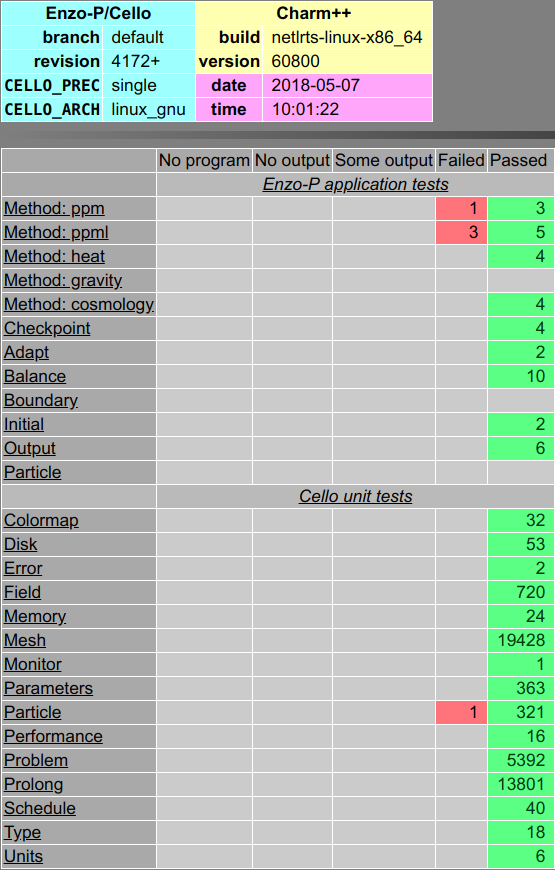
\includegraphics[width=1.75in]{Images/test-1.png}
\end{minipage} \ 
\begin{minipage}{2.25in}
\begin{itemize}
\item Summary of all tests
\item Columns:
\footnotesize
\begin{enumerate}
\item didn't compile
\item didn't start
\item didn't finish
\item tests failed
\item tests passed
\end{enumerate}
\small
\item A few failed tests are expected
\item Sections link to details
\end{itemize}
\end{minipage}
\end{frame}

%----------------------------------------------------------------------

\begin{frame}[fragile] 
\secframetitle{\ssTesting}
\framesubtitle{Enzo-P/Cello Test Results: adaptive mesh refinement}
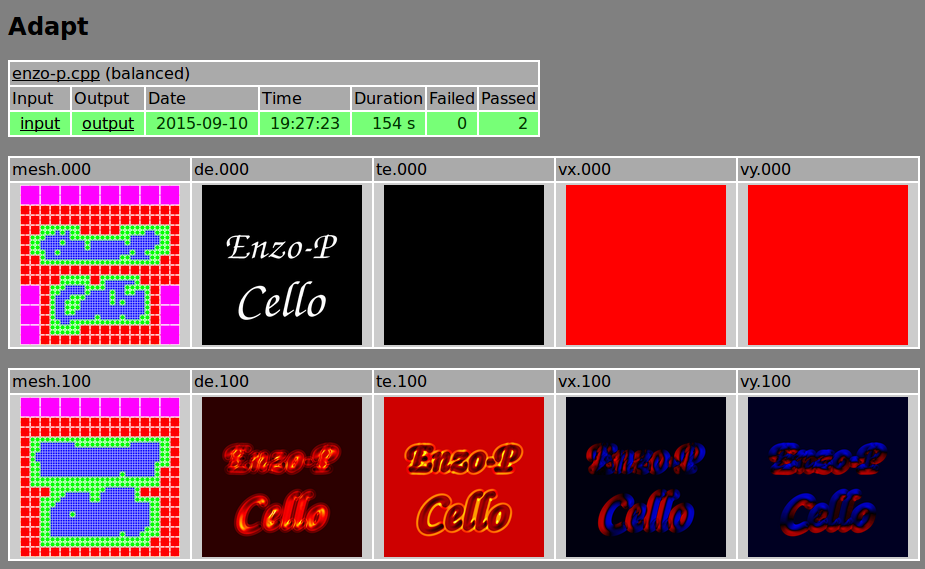
\includegraphics[width=4.0in]{Images/cello-test-2.png}
\end{frame}


\begin{frame}[fragile] 
\secframetitle{\ssTesting}
\framesubtitle{Enzo-P/Cello Test Results: dynamic load balancing}
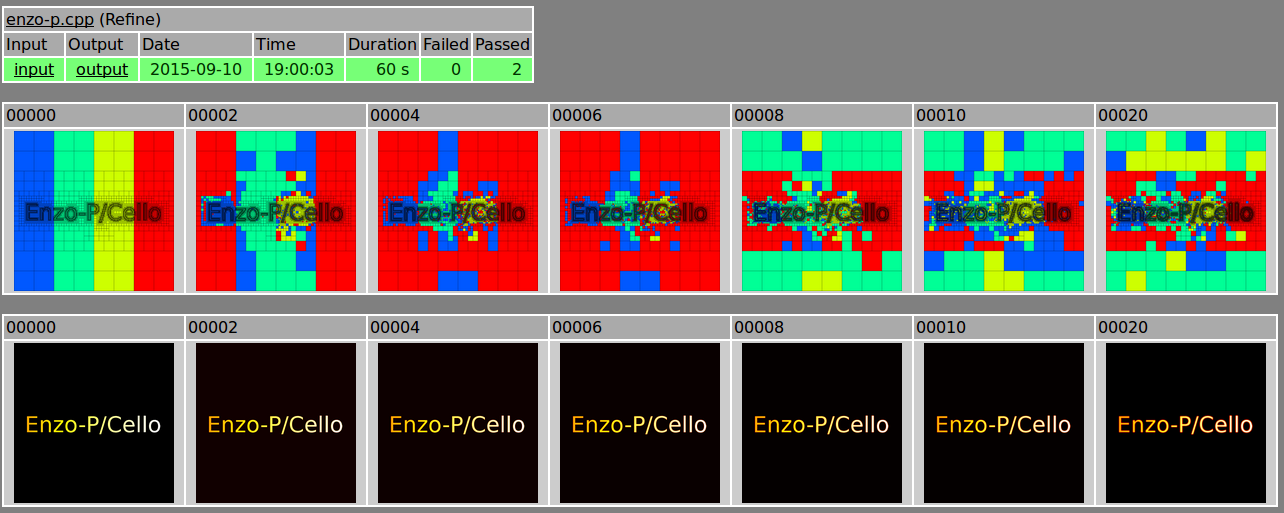
\includegraphics[width=4.0in]{Images/cello-test-3.png}
\end{frame}

 % How is testing done?
%======================================================================
\NEWSEC
%======================================================================

\subsection{\ssSource}

\begin{frame}[fragile,label=ss-source] 
\secframetitle{\ssSource}
\begin{itemize}
\item \greentext{\url{https://bitbucket.org/cello-project}}
\item \bluetext{Current project members} \\
\footnotesize
Michael Norman \\
James Bordner \\ 
Tom Abel \\
Greg Bryan \\
Dave Collins \\ 
Alexei Kritsuk \\ 
Brian O'Shea \\
Daniel Reynolds \\ 
Matthew Turk \\ 
John Wise \\
\normalsize
\item \bluetext{Repository:} \redcode{cello-src} \\
\small{\orangecode{hg clone ssh://hg@bitbucket.org/cello-project/cello-src}}
\end{itemize}
\end{frame}

\begin{frame}[fragile] 
\secframetitle{\ssSource}
\begin{itemize}
\item \bluetext{Basic directory structure: \redcode{cello-src/}\ldots} \\
\begin{tabular}{ll}
\redcode{src/Enzo} & \bluetext{Enzo-P source} \\
\redcode{src/Cello} & \bluetext{Cello source} \\
\redcode{bin/enzo-p} & \bluetext{executable} \\
\redcode{input} & \bluetext{sample parameter files} \\
\redcode{test} & \bluetext{tests and results} \\
\redcode{tools} & \bluetext{convenience utilities}
\end{tabular}
\item \bluetext{Some useful files} \\
\begin{tabular}{ll}
\redcode{build.sh} & \bluetext{Build script} \\
\redcode{SContstruct} & \bluetext{Top-level ``make'' file}\\
\redcode{errors.org} & \bluetext{Generated \code{org-mode} errors / warnings} \\
\redcode{diff.org} & \bluetext{Generated \code{org-mode} \greencode{hg diff}} \\
\redcode{log.org} & \bluetext{Generated \code{org-mode} \greencode{hg log}}
\end{tabular}

\end{itemize}
\end{frame}

 % Where is the source code hosted?
%======================================================================
\NEWSEC
%======================================================================

\subsection{\ssBrowse}

\begin{frame}[fragile,label=ss-browse] 
\secframetitle{\ssBrowse}
\begin{enumerate}
\item \bluetext{Bitbucket}
\begin{itemize}
\item \greentext{\url{https://bitbucket.org/cello-project/cello-src/src}}
\item \bluetext{good for viewing development history}
\end{itemize}
\item \bluetext{Doxygen on \code{cello-project.org} platform}
\begin{itemize}
\item \greentext{\url{http://cello-project.org/src}}
\item \bluetext{good for viewing annotated code structure}
\end{itemize}
\item \bluetext{Doxygen on your laptop}
\begin{itemize}
\item \redcode{make doc}
\item \greentext{\footnotesize\url{file:///home/bordner/Cello/cello-src/}\underline{src-html}\url{/index.html}}
\item \redcode{cd \underline{src-latex}; pdflatex refman.tex}
\end{itemize}
\end{enumerate}

\end{frame}

 % How can I browse the source code?
%======================================================================
\NEWSEC
%======================================================================

\subsection{\ssCommunicate}

\begin{frame}[fragile,label=ss-communicate] 
\secframetitle{\ssCommunicate}
\end{frame}

 % How do Enzo-P developers communicate?
